% !Mode:: "TeX:UTF-8"
%!TEX program  = xelatex
%中国光谷·“华为杯”第十九届中国研究生数学建模竞赛论文格式规范:
%论文题目和摘要写在论文摘要上,摘要页的下一页开始论文正文;
%论文从摘要页开始编写页码,页码必须位于每页页脚中部,用阿拉伯数字从“1 ”开始连续编号;
%论文题目用三号黑体字、一级标题用四号黑体字,并居中;
%论文中其他汉字一律采用小四号宋体字,行距用单倍行距。计算机结果和源程序需在规定时间内上传竞赛系统以备检查。
%请大家注意:摘要应该是一份简明扼要的详细摘要(包括关键词),请认真书写(注意篇幅一般不超过两页,且无需译成英文)。全国评阅时对摘要和论文都会审阅。
%论文不能有页眉,论文中不能有任何可能显示答题人身份的标志。

% “华为杯”第二十届中国研究生数学建模竞赛论文格式规范:
% 每个参赛队可以从A、B、C、D、E、F题中任选一题完成论文。
% 论文题目、摘要和关键词写在论文摘要页上,摘要页的下一页开始论文正文。
% 论文从摘要页开始编写页码,页码必须位于每页页脚中部,用阿拉伯数字从“1 ”开始连续编号。
% 论文不能有页眉,论文中不能有任何可能显示答题人身份的标志。
% 论文题目用三号黑体字、一级标题用四号黑体字,并居中。论文中其他汉字一律采用小四号宋体字,行距用单倍行距。如题目中有要求,计算机结果和源程序需在规定时间内上传竞赛系统以备检查。
% 请大家注意:摘要应简明扼要,需包含:建模思路、主要方法、模型、结果与结论、创新点、关键词等,请认真书写(注意篇幅一般不超过两页,且无需译成英文)。评阅时对摘要和论文都会审阅。
% 引用别人的成果或其他公开的资料(包括网上甚至在“博客”上查到的资料) 必须按照规定的参考文献的表述方式在正文引用处和参考文献中明确列出,引用程序须注明来源。正文引用处用方括号标示参考文献的编号,如[1][3]等;引用书籍还必须指出页码。参考文献按正文中的引用次序列出,其中书籍的表述方式为:
% [编号] 作者,书名,出版地:出版社,起止页码,出版年。
% 参考文献中期刊杂志论文的表述方式为:
% [编号] 作者,论文名,杂志名,卷期号:起止页码,出版年。
% 参考文献中网上资源的表述方式为:
% [编号] 作者,资源标题,网址,访问时间(年月日)。

%作者:图灵的猫 Qid:TuringsCat 邮箱:TuringsCat@126.com

\documentclass[a4paper]{CPIPC}


%--------------------正文----------------------
\begin{document}


\numberwithin{equation}{section}
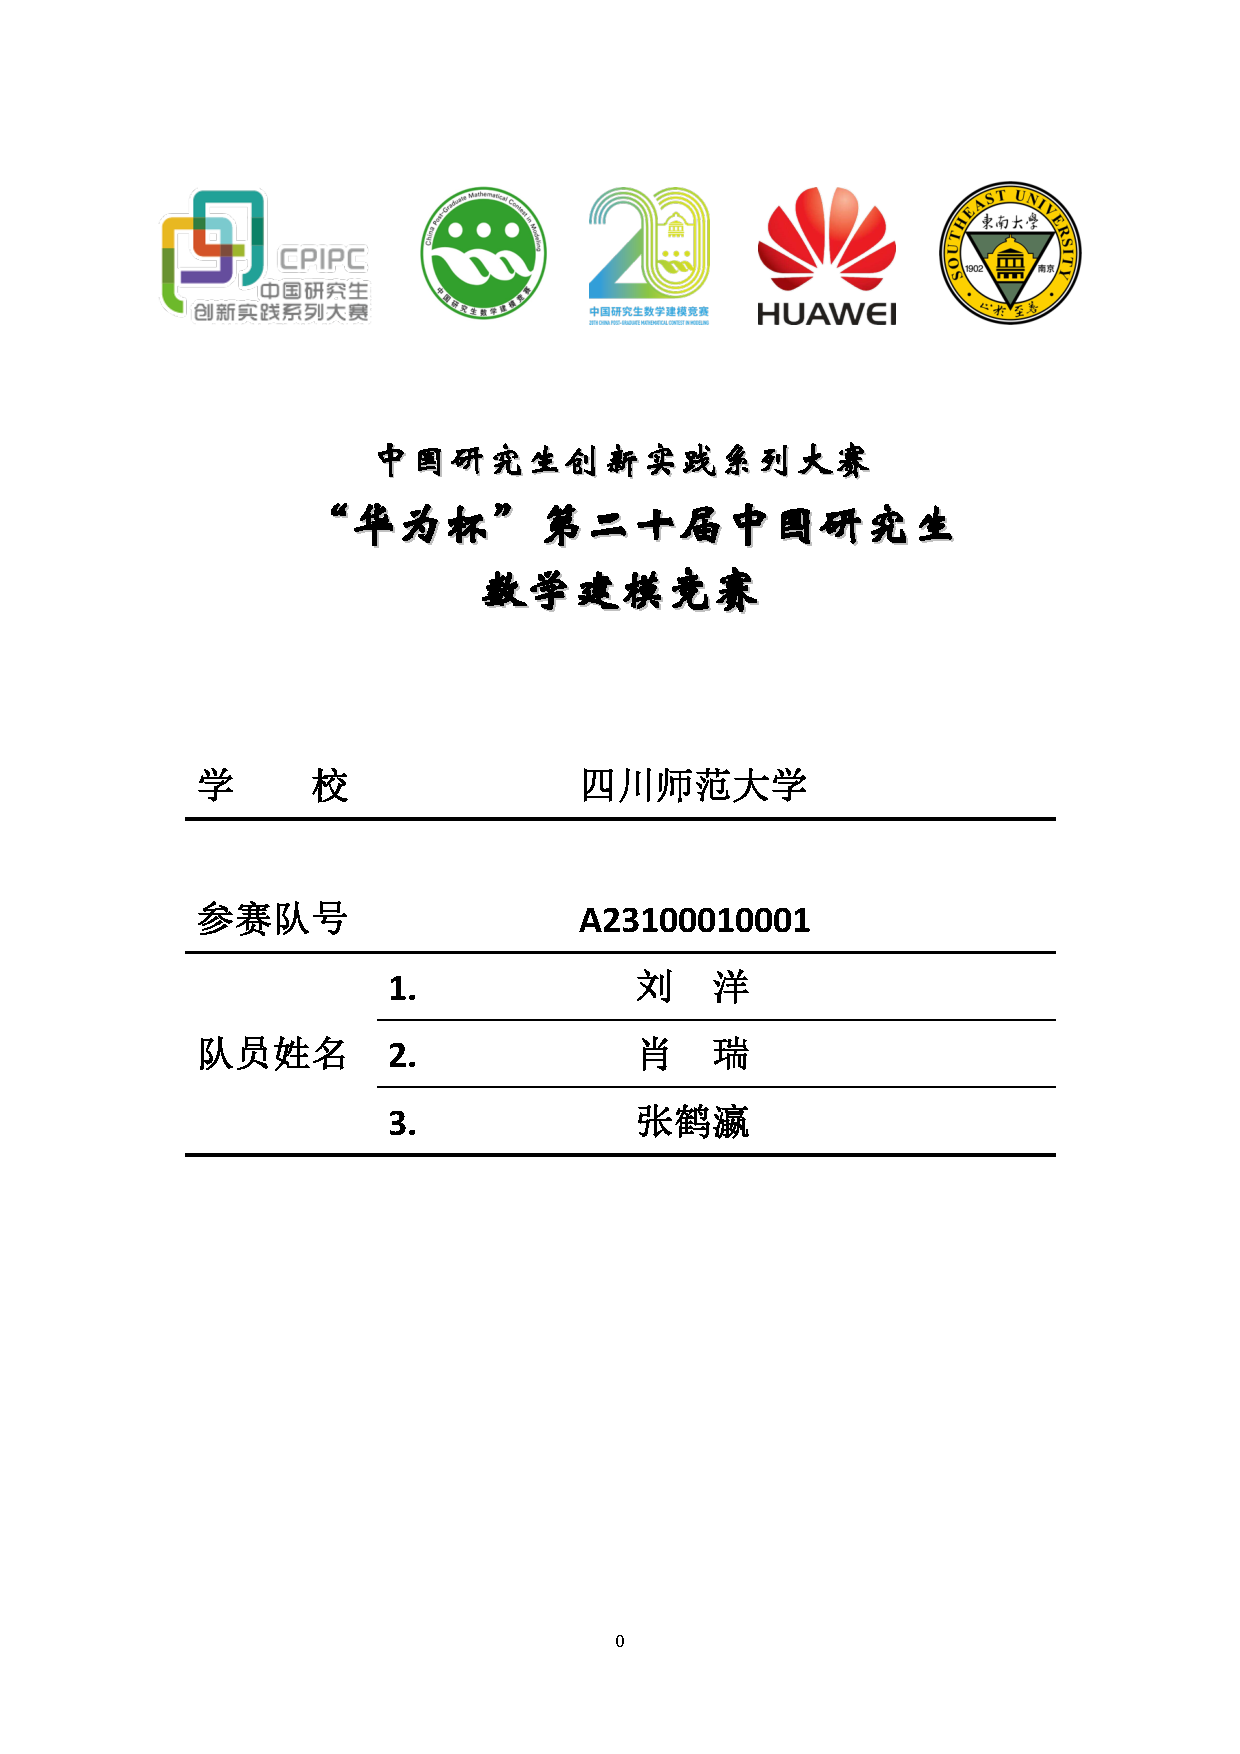
\includepdf[width=21cm]{section/titlepage/titlepage}

% --------------------题目&摘要页----------------------
%--------------------题目&摘要页----------------------
\newpage
\pagenumbering{arabic} %设置阿拉伯数字页码
\setcounter{page}{1} %正文为第一页

    \begin{center}
        \zihao{-2}  \bfseries \xinwei \shadowtext{中国研究生创新实践系列大赛}
    
        \zihao{2} \shadowtext{\textbf{ \xinwei “华为杯”第二十届中国研究生}}
    
        \zihao{2} \shadowtext{\textbf{\xinwei 数学建模竞赛}}
        \end{center}

\vspace{1em}
\begin{tabular}{l p{0.8\textwidth}<{\centering}}
    \centering
    \zihao{4} 题\quad 目\quad & \zihao{3} \heiti          \\ \cline{2-2}
\end{tabular}

\begin{center} \zihao{-2} \lishu 摘 \qquad 要:
\end{center}
% (此处填写摘要信息)
% \begin{enumerate}
%     \item 每个参赛队可以从A、B、C、D、E、F题中任选一题完成论文.
%     \item 论文题目和摘要写在论文摘要上,摘要页的下一页开始论文正文.
%     \item 论文从摘要页开始编写页码,页码必须位于每页页脚中部,用阿拉伯数字从“1 ”开始连续编号.
%     \item 论文不能有页眉,论文中不能有任何可能显示答题人身份的标志.
%     \item 论文题目用三号黑体字、一级标题用四号黑体字,并居中.论文中其他汉字一律采用小四号宋体字,行距用单倍行距.计算机结果和源程序需在规定时间内上传竞赛系统以备检查.
%     \item 请大家注意:摘要应该是一份简明扼要的详细摘要(包括关键词),请认真书写(注意篇幅一般不超过两页,且无需译成英文).全国评阅时对摘要和论文都会审阅.
%     \item 引用别人的成果或其他公开的资料(包括网上甚至在“博客”上查到的资料) 必须按照规定的参考文献的表述方式在正文引用处和参考文献中明确列出.正文引用处用方括号标示参考文献的编号,如\cite{ref1}\cite{ref2}等;引用书籍还必须指出页码.参考文献按正文中的引用次序列出,其中书籍的表述方式为:
%     [编号] 作者,书名,出版地:出版社,起止页码,出版年.
%     参考文献中期刊杂志论文的表述方式为:
%     [编号] 作者,论文名,杂志名,卷期号:起止页码,出版年.
%     参考文献中网上资源的表述方式为:
%     [编号] 作者,资源标题,网址,访问时间(年月日).
% \end{enumerate}


  
    
\vspace{1em}
\noindent \textbf{关键词:} 


%--------------------目录----------------------
%--------------------目录----------------------
\newpage

\begin{center}
\tableofcontents
\end{center}


%--------------------正文----------------------
%--------------------问题重述----------------------

%--------------------问题重述----------------------
\newpage
\section{问题重述}


%--------------------问题分析----------------------

%--------------------问题分析----------------------


\section{问题分析}


%--------------------模型假设----------------------
\section{模型假设}


%--------------------符号说明----------------------
%--------------------符号说明----------------------
\section{符号说明}

%使用三线表格最好~
    % \begin{table}[H]
    %     \centering
    %     \caption{符号说明}
    %     \begin{tabularx}{\textwidth}{@{}lXl@{}}
    %         \toprule
    %         \textbf{符号} & \textbf{定义} & \textbf{单位} \\
    %         \midrule
    %         $j$ & 景点的索引号 & - \\
    %         $\omega_{j}$ & 景点 $j$ 的综合游玩价值 & - \\
    %         $\omega_{\text{用户},j}$ & 景点 $j$ 的用户评分 & 无 \\
    %         $\omega_{\text{历史},j}$ & 景点 $j$ 的历史与文化价值 & 无 \\
    %         $\omega_{\text{自然},j}$ & 景点 $j$ 的自然风光价值 & 无 \\
    %         $\omega_{\text{饮食},j}$ & 景点 $j$ 的饮食文化价值 & 无 \\
    %         $\omega_{\text{人流量},j}$ & 景点 $j$ 的日均人流量 & 无 \\
    %         $\alpha, \beta, \gamma, \delta, \epsilon$ & 权重系数 & - \\
    %         $D_{ij}$ & 从景点 $i$ 到景点 $j$ 的路程 & \si{\kilo\meter} \\
    %         $T_{ij}$ & 从景点 $i$ 到景点 $j$ 的预估旅行时间 & \si{\hour} \\
    %         $t_j$ & 景点 $j$ 的推荐参观时间 & \si{\hour} \\
    %         $x_{ij}$ & 从景点 $i$ 到景点 $j$ 的决策变量 & 无 \\
    %         $P_{\text{总}}$ & 总预算 & 元 \\
    %         $P_{\text{住}}$ & 日均住宿费用 & 元/天 \\
    %         $P_{\text{其}}$ & 日均其他费用 & 元/天 \\
    %         $P_{\text{行}ij}$ & 从景点 $i$ 到景点 $j$ 的交通费用 & 元 \\
    %         $P_{\text{票}j}$ & 景点 $j$ 的门票费用 & 元 \\
    %         $P_{\text{景}j}$ & 在景点 $j$ 的平均消费(门票除外) & 元 \\
    %         \bottomrule
    %     \end{tabularx}
    %     \label{table:symbol-definitions}
    % \end{table}

%--------------------模型建立与求解----------------------
%--------------------模型建立与求解----------------------

\section{模型建立与求解}


%--------------------模型评价----------------------
%--------------------模型评价----------------------
\section{模型评价与拓展}

\subsection{模型评价}

\subsubsection{模型优势}


\subsubsection{模型局限}


\subsection{模型拓展与前景}



%--------------------参考文献----------------------

%--------------------参考文献----------------------
\addcontentsline{toc}{section}{参考文献} %将参考文献放进目录

\begin{thebibliography}{99}
    
    % \bibitem{zhang2019}
    % 张岐山, 张兴婷. 基于签到数据和交通工具的多目标旅游路线推荐[J]. 西安电子科技大学学报(社会科学版), 2019.

    % \bibitem{he2020}
    % 贺剑武. 基于大数据分析技术的旅游智慧平台设计[J]. 现代电子技术, 2020.

    % \bibitem{teng2017}
    % 滕泉, 沈景凤, 徐斌. 基于贪婪算法的旅游路线优化问题[J]. 电子科技, 2017, 30(09): 142-145.

    % \bibitem{wu2021}
    % 武海涛. 基于多约束多目标的旅游路线规划研究与实现[D]. 中南财经政法大学, 2021.

    % \bibitem{yang2022}
    % 杨德青. 一种基于自驾游路线规划的多目标优化算法[J]. 信息技术与信息化, 2022, (05): 197-200.

    % \bibitem{ji2022}
    % 季亚龙. 基于蚁群改进算法的游客路线规划的研究[D]. 广西大学, 2023.

    % \bibitem{chui2022}
    % 崔贯娇. 基于时空深度学习的快递员揽件路线推荐方法研究[D]. 北京交通大学, 2022.

\end{thebibliography}


%--------------------附录----------------------

%--------------------附录----------------------
\newpage

\appendix

\section{主程序源代码}

\subsection{\texttt{DirectedGraphVisualization.m}}\label{sec A 4}
这段代码主要用于生成一个有向图并进行可视化。
\begin{lstlisting}[style=matlab,basicstyle=\footnotesize\fontspec{Courier New},title={DirectedGraphVisualization.m}]  
    % 设置随机数生成器的种子以获得可重复的结果
    rng(3);
    
    % 定义节点数量
    numNodes = 5;
    
    % 随机生成边(每个节点都可以连接到其他节点,但不包括自己)
    s = repmat(1:numNodes, 1, numNodes);
    t = repmat(1:numNodes, numNodes, 1);
    s = s(:)';
    t = t(:)';
    
    % 删除自连接的边
    selfLoops = s == t;
    s(selfLoops) = [];
    t(selfLoops) = [];
    
    % 随机生成边的权重和节点的权重
    edgeWeights = round((0.01 + (1-0.01)*rand(1, length(s))) * 100) / 100;
    nodeWeights = randi([20, 50], 1, numNodes);
    
    % 使用边和权重创建有向图对象
    G = digraph(s,t,edgeWeights);
    
    % 绘制有向图,并明确不显示节点标签
    h = plot(G, 'EdgeLabel', G.Edges.Weight, 'LineWidth', 2, 'ArrowSize', 10, 'NodeFontSize', 12, 'NodeColor', Color_Nature(1,:), 'EdgeColor', Color_Nature(2,:), 'EdgeAlpha', 0.7, 'ArrowPosition', 0.6, 'NodeLabel', {});
    
    % 使用节点的权重来调整节点的大小
    h.MarkerSize = nodeWeights;
    
    % 获取节点的坐标
    x = h.XData;
    y = h.YData;
    
    % 添加编号到节点的中心
    labels = arrayfun(@(x) num2str(x), 1:numNodes, 'UniformOutput', false);
    for i = 1:numNodes
        text(x(i), y(i), labels{i}, ...
            'HorizontalAlignment', 'center', ...
            'VerticalAlignment', 'middle', ...
            'Color', Color_Nature(3,:), ...
            'FontSize', 14, ...  % 设置字体大小,您可以根据需要调整
            'FontWeight', 'bold');  % 设置为加粗
    end

\end{lstlisting}


\end{document}